\documentclass[a4paper,12pt]{report}

\usepackage[italian]{babel}
\usepackage[utf8]{inputenc}
\usepackage[T1]{fontenc}
\usepackage{graphicx}
%\usepackage[style=numeric-comp]{biblatex}

\title{InfoTreno}
\author{Chelli M. \thanks{michael.chelli@studio.unibo.it - 915585}, Tampieri E.\thanks{eugenio.tampieri@studio.unibo.it - 915602} - Gruppo 2098}

\begin{document}
	\maketitle
	\tableofcontents
	\chapter{Analisi dei requisiti}
	\section{Intervista}
	\par RFS (Rete Ferroviaria dello Stato) richiede la realizzazione di un sistema informativo in grado di monitorare la marcia e la programmazione dei treni e la gestione dei turni del personale di bordo. Viene richiesta la possibilità di operare tramite interfaccia web, in modo da essere indipendenti dalle piattaforme utilizzate.
	\par Un treno è uno specifico viaggio su una relazione, ovvero l'attraversamento sequenziale di una serie di punti di passaggio (scambi, stazioni, o semplici) in orari predeterminati.
	\par Oltre alla memorizzazione degli orari di attraversamento teorici, viene richiesta la memorizzazione della data e ora di partenza e di arrivo da un punto di passaggio, così da poter calcolare il ritardo del treno.
	\par Un treno è poi composto da una locomotiva (della quale ci interessa conoscere la velocità e la tensione di esercizio) e una serie di carrozze (delle quali ci interessa memorizzare la classe e il numero di posti), che formano un convoglio.
	\par Su un treno prendono servizio un macchinista, un capotreno e, in certi casi, dei controllori.

	\section{Rilevamento delle ambiguità e correzioni proposte}
	\par RFS (Rete Ferroviaria dello Stato) richiede la realizzazione di un sistema informativo in grado di monitorare la marcia e la programmazione dei treni e la gestione dei turni del personale di bordo. Viene richiesta la possibilità di operare\textsuperscript{1} tramite interfaccia web, in modo da essere indipendenti dalle piattaforme utilizzate.
	\par Un treno è uno specifico viaggio su una linea ferroviaria, ovvero l'attraversamento sequenziale di una serie di punti di passaggio\textsuperscript{2} (scambi, stazioni, o semplici\textsuperscript{3}) in orari predeterminati.
	\par Oltre alla memorizzazione degli orari di attraversamento teorico, viene richiesta la memorizzazione della data e ora di partenza e di arrivo da un punto di passaggio, così da poter calcolare il ritardo del treno.
	\par Un treno è poi composto da una locomotiva (della quale ci interessa conoscere la velocità e la tensione di esercizio) e una serie di carrozze (delle quali ci interessa memorizzare la classe\textsuperscript{4} e il numero di posti), che formano un convoglio.
	\par Su un treno prendono servizio un macchinista, un capotreno e, in certi casi, dei controllori.

	\begin{tabular}{|p{1cm}|p{3cm}|p{4cm}|p{4cm}|}
		\hline
		\textbf{N} & \textbf{Espressione} & \textbf{Sostituzione} & \textbf{Motivazione} \\ \hline
		1 & Operare & Interagire con il sistema & Esplicitato il concetto  \\ \hline
		2 & Punti di passaggio & rappresentati nel mondo fisico da eurobalise & specificato il significato \\ \hline
		3 & Semplici & in tutti gli altri casi & specificato il significato \\ \hline
		4 & classe & classe (prima o seconda) & specificato il significato \\ \hline
	\end{tabular}

	\subsection{Dopo la correzione delle ambiguità}
	\par RFS (Rete Ferroviaria dello Stato) richiede la realizzazione di un sistema informativo in grado di monitorare la marcia e la programmazione dei treni e la gestione dei turni del personale di bordo. Viene richiesta la possibilità di interagire con il sistema tramite interfaccia web, in modo da essere indipendenti dalle piattaforme utilizzate.
	\par Un treno è uno specifico viaggio su una linea ferroviaria, ovvero l'attraversamento sequenziale di una serie di punti di passaggio, rappresentati nel mondo fisico da eurobalise (scambi, stazioni, o semplici, in tutti gli altri casi) in orari predeterminati.
	\par Oltre alla memorizzazione degli orari di attraversamento teorico, viene richiesta la memorizzazione della data e ora di partenza e di arrivo da un punto di passaggio, così da poter calcolare il ritardo del treno.
	\par Un treno è poi composto da una locomotiva (della quale ci interessa conoscere la velocità e la tensione di esercizio) e una serie di carrozze (delle quali ci interessa memorizzare la classe, prima o seconda, e il numero di posti), che formano un convoglio.
	\par Su un treno prendono servizio un macchinista, un capotreno e, in certi casi, dei controllori.

	\section{Definizione delle specifiche in linguaggio naturale ed estrazione dei concetti principali}
	\par Si individuano le parole chiave che permetteranno di costruire un primo schema scheletro del progetto. In seguito sarà poi raffinato per ottenere lo schema definitivo. I termini essenziali sono evidenziati in grassetto e in corsivo.
	\par RFS (Rete Ferroviaria dello Stato) richiede la realizzazione di un sistema informativo in grado di monitorare la marcia e la programmazione dei treni e la gestione dei turni del personale di bordo. Viene richiesta la possibilità di interagire con il sistema tramite interfaccia web, in modo da essere indipendenti dalle piattaforme utilizzate.
	\par Un \textbf{\textit{treno}} è uno specifico viaggio su una linea ferroviaria, ovvero l'attraversamento sequenziale di una serie di \textbf{\textit{punti di passaggio}}, rappresentati nel mondo fisico da eurobalise (scambi, stazioni, o semplici, in tutti gli altri casi) in orari predeterminati.
	\par Oltre alla memorizzazione degli \textbf{\textit{orari di attraversamento}} teorico, viene richiesta la memorizzazione della \textbf{\textit{data e ora di partenza e di arrivo}} da un punto di passaggio, così da poter calcolare il ritardo del treno.
	\par Un treno è poi composto da una \textbf{\textit{locomotiva}} (della quale ci interessa conoscere la velocità e la tensione di esercizio) e una serie di \textbf{\textit{carrozze}} (delle quali ci interessa memorizzare la classe (prima o seconda) e il numero di posti), che formano un \textbf{\textit{convoglio}}.
	\par Su un treno prendono servizio un macchinista, un capotreno e, in certi casi, dei controllori.
% ____                           _   _               _
%|___ \  ___ ___  _ __   ___ ___| |_| |_ _   _  __ _| | ___
%  __)  / __/ _ \| '_ \ / __/ _ | __| __| | | |/ _` | |/ _ \
% / __/| (_| (_) | | | | (_|  __| |_| |_| |_| | (_| | |  __/
%|_____ \___\___/|_| |_|\___\___|\__|\__|\__,_|\__,_|_|\___|
	\chapter{Progettazione concettuale}
	\par In questa situazione il dominio è specifico ed è spesso possibile trovare delle entità generiche che si concretizzano poi in entità più specifiche. Per questo motivo è utile utilizzare un approccio top-down per modellare al meglio l'architettura.
	\section{Schema scheletro}
	\begin{figure}[h]
		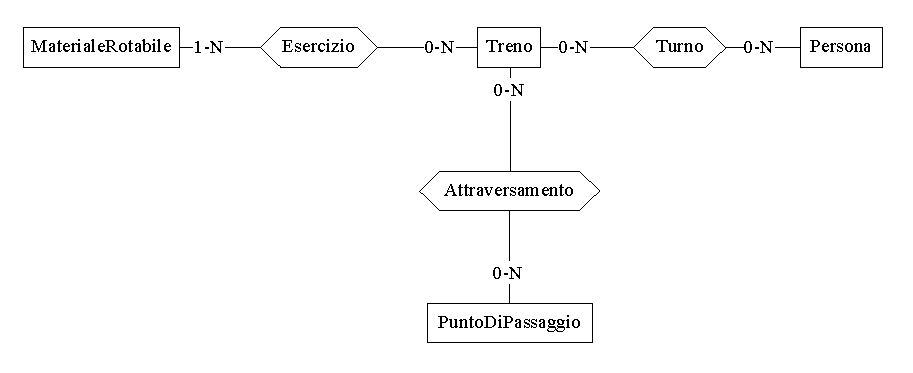
\includegraphics[width=\linewidth]{res/schema/skel}
		\caption{Schema scheletro}
	\end{figure}
	\section{Raffinamenti proposti}
	\par Lo schema concettuale sarà sviluppato perfezionando tutte le entità nello schema scheletro. Per ogni entità si propone di seguito una vista esplosa, l’unione delle quali condurrà allo schema finale.
	\subsection{Entità \textit{MaterialeRotabile}}
	\begin{figure}[h]
		\begin{center}
			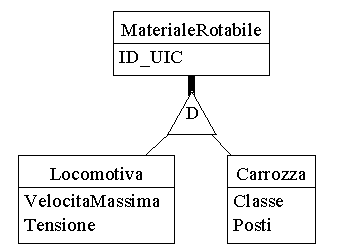
\includegraphics{res/schema/loco}
		\end{center}
		\caption{Gerarchia di MaterialeRotabile}
		\label{fig:loco}
	\end{figure}
	\par Il materiale rotabile viene suddiviso in locomotive e carrozze (fig. \ref{fig:loco}), lasciando eventualmente spazio ad altri tipi di materiale rotabile quali i carri merci.
	\par Al contempo, si vuole differenziare la relazione fra una carrozza e una locomotiva, facendo in modo che ci possa essere solo una locomotiva per ogni convoglio (fig. \ref{fig:esercizio}). Per ottenere ciò viene aggiunta una entità chiamata \textit{Convoglio}, alla quale vengono messi in relazione una \textit{Locomotiva} e zero o più \textit{Carrozze}. Alla fine del raffinamento, viene sostituita la relazione fra \textit{Treno} e \textit{MaterialeRotabile} con una relazione fra \textit{Treno} e \textit{Convoglio} che a sua volta è collegato alle entità gerarchicamente figlie di \textit{Materiale rotabile}.
	\begin{figure}[h]
		\begin{center}
			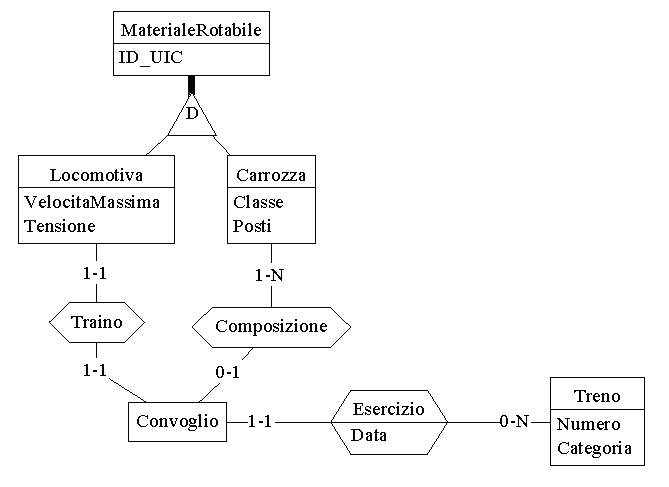
\includegraphics{res/schema/esercizio}
		\end{center}
		\caption{La relazione esercizio con le relative entità}
		\label{fig:esercizio}
	\end{figure}
	\subsection{Entità}
	\section{Schema concettuale finale}
	\begin{figure}
		\begin{center}
			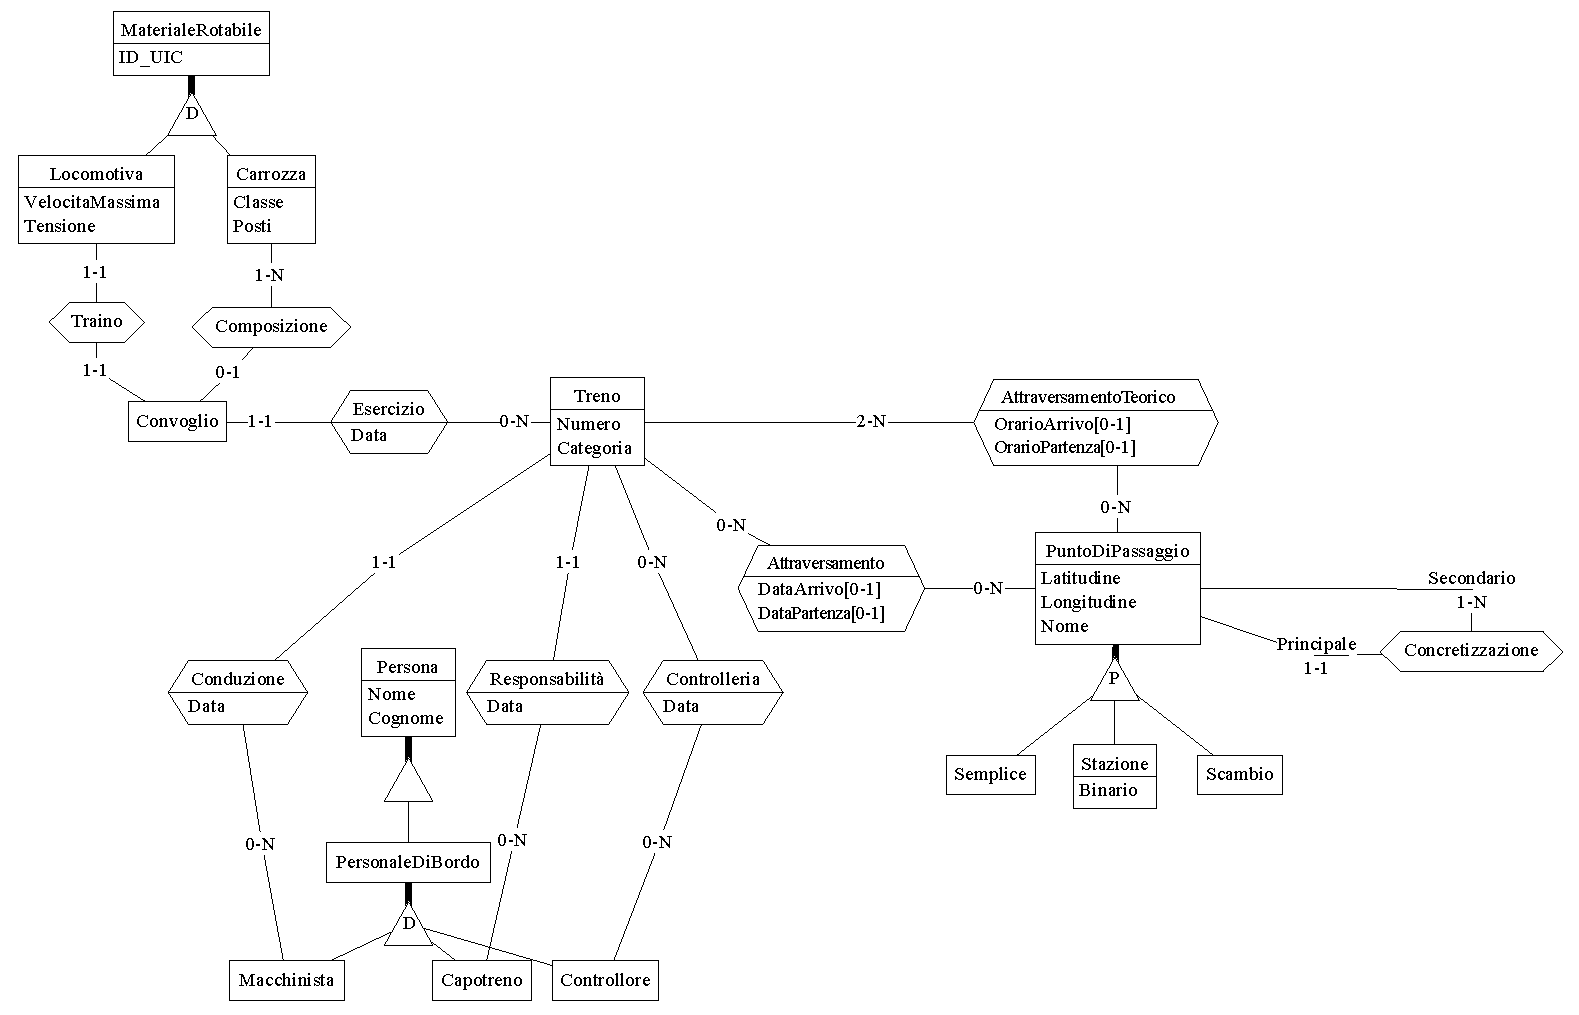
\includegraphics[angle=270,width=.95\linewidth]{res/schema/full}
		\end{center}
		\caption{Schema concettuale}
	\end{figure}
	\chapter{Progettazione logica}
	\section{Stima del volume dei dati}
	\par Si ripoerao le stime dei volumi dei dati dopo un anno di operatività.
	\begin{table}
	\centering
	\begin{tabular}{|l|l|l|}
		\hline
		Nome & Tipo & Volume \\
		\hline
		     &      &        \\
		\hline
		     &      &        \\
		\hline
		     &      &        \\
		\hline
	\end{tabular}
	\end{table}
	\section{Descrizione delle operazioni principali e stima della loro frequenza}
	\section{Schemi di navigazione e tabelle degli accessi}
	\subsection{Schemi di navigazione}
	\subsection{Tabella degli accessi}
	\section{Raffinamento dello schema (eliminazione di identificatori esterni, attributi composti e gerarchie, scelta delle chiavi)}
	\subsection{Eliminazione delle gerarchie}
	\subsection{Attributi composti}
	\subsection{Scelta delle chiavi primarie}
	\subsection{Chiavi esterne}
	\subsection{Vincoli di gruppo}
	\subsection{Accorgimenti}
	\section{Analisi delle ridondanze}
	\section{Traduzione di entità e associazioni in relazioni}
	\section{Schema relazionale finale}
	\section{Traduzione delle operazioni in query SQL}
	\chapter{Progettazione dell'applicazione}
	
	\section{Descrizione dell'architettura dell'applicazione realizzata}
	\subsection{Homepage}
	\subsection{Ricerca treno}
	\subsection{Ricerca stazione...}
	\appendix
	\chapter{Istruzioni per l'installazione}
	\section{Prerequisiti}
	\begin{itemize}
		\item Un DBMS PostgreSQL con già creato un database vuoto
		\item Un utente che abbia i permessi di creazione tabelle e viste, di interrogazione e di inserimento sul database
	\end{itemize}
	\section{Configurazione}
	\par \`E necessario creare un file denominato \texttt{.env} nella cartella in cui verrà eseguito il programma, contenente nel formato \texttt{<KEY>=<VALUE>} (una variabile per riga) le seguenti variabili:
	\begin{itemize}
		\item \texttt{DB\_HOST}: l'indirizzo IP o l'hostname su cui è raggiungibile il DBMS,
		\item \texttt{DB\_NAME}: il nome del DB in cui verranno create le tabelle,
		\item \texttt{DB\_USER}: l'utente per autenticarsi al DB,
		\item \texttt{DB\_PASSWORD}: la password dell'utente sopra specificato.
	\end{itemize}
	\section{Esecuzione del programma}
	\par Dopo aver scaricato l'eseguibile per la piattaforma desiderata, controllare che abbia i permessi di esecuzione (se richiesti) ed eseguirlo nella cartella in cui è stato posizionato il file \texttt{.env} e la cartella \texttt{templates}.
	\par Il programma provvederà all'inizializzazione del DB e si metterà in ascolto sulla porta TCP 8000.
    %\printbibliography[heading=bibintoc]
    \listoffigures
\end{document}
